\section{Trabalhos Relacionados}\label{sec:rel}

A literatura em redução de dimensionalidade é extensa e os métodos desenvolvidos apresentam grande diversidade em relação a aspectos matemáticos e computacionais. Buscando uma melhor contextualização, esta seção aborda apenas trabalhos que buscam de alguma forma utilizar representações visuais para a execução desta tarefa.

Em visualização computacional a redução de dimensionalidade pode ser realizada seguindo duas abordagens. A primeira delas busca compor um subconjunto das dimensões originais que contém atributos realmente relevantes para a análise. Por manterem o significado dos atributos originais, essas técnicas são análogas aos métodos automáticos de seleção de características e por isso herdam esta nomenclatura. Já a segunda abordagem, parte dos princípios dos métodos automáticos de combinação de características, os quais criam um novo conjunto de dimensões que tenta conservar as propriedades e relacionamentos do conjunto original.

\subsection{Seleção de Características}

% VHDR & DOSFA %%%%

% Em busca de construir espaços de baixa dimensionalidade mais intuitivamente do que pelo uso de métodos automáticos, \citeauthor{Yang2003} desenvolveram um método de redução de dimensionalidade chamado VHDR (Visual Hierarchical Dimensions Reduction)~\cite{Yang2007}. Este método utiliza a similaridade entre pares de dimensões para construir uma organização hierárquica dos atributos. O processo é ortogonal ao agrupamento de itens, assim é possível identificar grupos de dimensões com características semelhantes. Porém, para conjuntos de dados com mais do que algumas dezenas de dimensões, as representações visuais utilizadas podem se tornar poluídas. Os autores mencionam que algoritmos adaptados da área de agrupamentos de dados poderiam ser utilizados para gerar a hierarquia de dimensões, no entanto eles adotaram uma abordagem mais simples para medir a similaridade entre dimensões: medem a diferença entre os valores normalizados dos atributos e verificam se esta diferença é menor do que um \textit{threshold} pré estabelecido. Este método para o cálculo da similaridade é a grande limitação do trabalho, pois não captura dependências entre os atributos. Além disso, não são apresentadas mecanismos interativos como alternativa para o método automático de identificação de dimensões representativas de um grupo. 

% The Dimension Ordering Spacing and Filtering Approach (DOSFA) [26] has evolved from VHDR and provides di- mensionality reduction based on a combination of similarity and of a given importance measure, such as variance. DOSFA is also aiming at finding a visual layout that facilitate the detection of structures within the data.

Em busca de construir espaços de baixa dimensionalidade mais intuitivamente do que pelo uso de métodos automáticos, \cite{Yang2003} e \cite{Ward2003} constroem uma hierarquia com base na similaridade entre as dimensões para apresentar explicitamente os relacionamentos entre os atributos e permitem que os usuários interativamente selecionem as dimensões de interesse. 

% O processo é ortogonal ao agrupamento de itens, assim é possível identificar grupos de dimensões com características semelhantes. Porém, para conjuntos de dados com mais do que algumas dezenas de dimensões, as representações visuais utilizadas podem se tornar poluídas. Os autores mencionam que algoritmos adaptados da área de agrupamentos de dados poderiam ser utilizados para gerar a hierarquia de dimensões, no entanto eles adotaram uma abordagem mais simples para medir a similaridade entre dimensões: medem a diferença entre os valores normalizados dos atributos e verificam se esta diferença é menor do que um \textit{threshold} pré estabelecido. Este método para o cálculo da similaridade é a grande limitação do trabalho, pois não captura dependências entre os atributos. Além disso, não são apresentadas mecanismos interativos como alternativa para o método automático de identificação de dimensões representativas de um grupo. 

% Corrgram e  Coord %%%%

% Coord aborda o problema de que subconjuntos dos dados podem apresentar características diferentes, assim em alguns casos é impossível encontrar um único conjunto de atributos que represente todos os subconjuntos adequadamente. 

Quando o número de dimensões está na casa das centenas ou dezenas, não é possível inspecionar todas as dimensões exaustivamente. Assim, métodos estatísticos são utilizados para fornecer medidas de comparação entre os atributos. Entre essas medidas, as mais utilizadas são medidas de correlação estatística.

Medidas de correlação são normalmente apresentadas com o auxílio de uma matriz de correlação~\cite{Friendly2002}. Este tipo de representação é útil para se ter uma visão geral das relações entre pares de elementos e permite que um grande número de itens seja analisado. No entanto, para análises mais detalhadas, ou que exijam uma comparação entre mais do que simplesmente pares de elementos, não é uma representação adequada.
% RBF %%%%

\citeauthor{Shneiderman2004} desenvolveram o framework Rank-by-Feature~\cite{Shneiderman2004} com o intuito de auxiliar a descoberta de correlações entre atributos. Eles classificam os atributos com base em critérios estatísticos definidos pelo usuário e possibilitam a construção de projeções uni ou bidimensionais para a avaliação da classificação realizada. 

% Certas análises podem exigir demasiado esforço do usuário, devido à necessidade de se explorar individualmente cada dimensão ou avaliar par a par as relações entre atributos. Com a ocorrência de dependências não lineares este problema torna-se ainda maior e o usuário pode facilmente se perder em suas análises e não extrair novos conhecimentos dos resultados.

% Smart stripes e Guiding %%%%

\cite{May2011} parte da ideia introduzida em \cite{May2011ss} para propor uma técnica para avaliação e orientação do processo de feature selection com base em métodos interativos visuais. Trata o problema de que diferentes partições das entidades dos dados podem apresentar  importâncias distintas de features. Permite que o usuário participe do processo de seleção e a investigue as dependências e interdependências entre conjuntos de features e itens.

% Um problema desta técnica é a necessidade de se estabelecer uma feature de referência, pois a representação visual apresenta apenas as relações de 1-n.

\subsection{Combinação de Características}

% Existem três principais abordagens para se reduzir a dimensionalidade dos conjuntos de dados a partir da combinação dos atributos. Análise de Componentes Principais (\textit{Principal Component Analysis)}~ ou simplesmente PCA, realiza combinações lineares sobre os atributos de modo que o novo espaço agregue a maior parte da variância dos dados. Para análises onde relações não lineares devem ser consideradas, \textit{Multimensional Scaling} (MDS) é uma alternativa interessante, pois trata-se de um algoritmo de otimização iterativo não linear, que busca minimizar as distâncias entre os elementos no espaço projeto e no espaço original. A área de aprendizado de máquina contribuiu com o método não supervisionado \textit{Self Organizing Maps} (SOM) para transformar conjuntos de dados em mapas bidimensionais.

% PCA methods can only work well for linear relationships.
% The impact of every original dimension is more or less still there.
% Scalability to high dimensionality. Although efficient algorithms for K-means or EM-based clustering have been developed repeatedly using such clustering algorithms to evaluate a large number of candidates (i.e., subsets of dimensions) can still cause computational efficiency problems, especially when both d and n are large.

Ao lidar com dados de alta dimensionalidade, costuma-se preceder a visualização com métodos ``caixa-preta'' como \textit{Principal Component Analysis} (PCA)~\cite{Wold1987},  \textit{Multimensional Scaling} (MDS)~\cite{Mead1992} ou \textit{Self Organizing Maps} (SOM)~\cite{Kohonen1990}. Apesar de popular, esta abordagem não utiliza os conceitos da área de visualização ao seu favor, pois o usuário não participa na etapa crucial da geração dos resultados, a redução de dimensionalidade.

% PCA is not effective in identifying relationships or patterns that reside in different subspaces. SOM uses measurements from all original dimensions to derive the projection to a 2-D space and therefore noisy or irrelevant dimensions have dramatic impacts on the projection result

Existem trabalhos que buscam contornar esse problema ao incluir a participação do usuário nesses métodos e tornar essas ``caixas pretas'' mais compreensivas. A técnica iPCA~\cite{Jeong2009}, por exemplo, provém meios para o usuário manipular os parâmetros da técnica PCA e, assim, ser capaz de entender mais facilmente as transformações realizadas sobre os dados. Similarmente, MDSteer [24] permite que o usuário guie o processo de MDS ao escolher regiões de interesse para se concentrar os esforços computacionais. No entanto, os mecanismos de interação propostos por esses trabalhos se baseiam em interfaces que são demasiadamente complexas ou que não contém todos os mecanismos necessários para lidar com um grande volume de dados.

Métodos mais sofisticados têm sido desenvolvidos para lidar com as novas exigências impostas pelos grandes conjuntos de dados e que se preocupam em fornecer interfaces intuitivas aos usuários. Estes métodos combinam diversas técnicas em um sistema integrado e possibilitam a interação do usuário para viabilizar a exploração de conjuntos de dados que possuem um elevado número de atributos.

% VAR %%%%

A técnica VaR (Value and Relation)~\cite{Yang2004}, por exemplo, une os conceitos de MDS e glifos para representar as dependências das dimensões de uma base de dados. Como mostra a Figura~\ref{fig:var1}, cada glifo representa uma dimensão e de acordo com seus posicionamentos no plano, o usuário pode compreender quais dimensões se relacionam entre si e assim, pode escolher somente atributos de real interesse e não redundantes para análises mais detalhadas.

\begin{figure}[h!]
  \centering
  \begin{subfigure}[b]{0.5\textwidth}
    \centering
    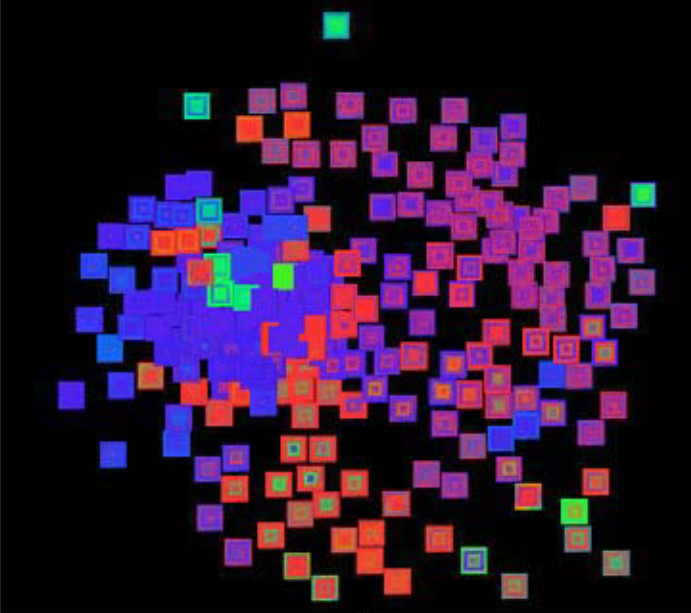
\includegraphics[width=\textwidth]{images/var1.png}
    \caption{}
    \label{fig:var1}
  \end{subfigure}%
  ~ %add desired spacing between images, e. g. ~, \quad, \qquad etc.
  \begin{subfigure}[b]{0.475\textwidth}
    \centering
    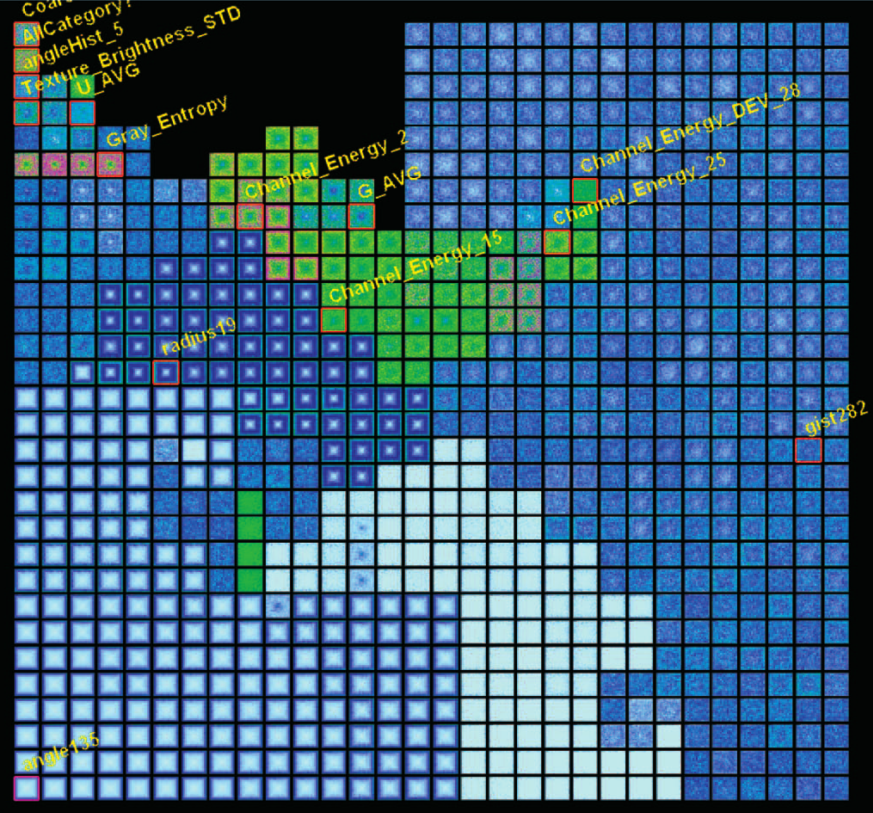
\includegraphics[width=\textwidth]{images/var2.png}
    \caption{}
    \label{fig:var2}
  \end{subfigure}
  \caption[VaR: Value and Relation]{(a) Exemplo da técnica VaR para um conjunto de $50.000$ itens e $361$ dimensões. Cada dimensão é representada por um glifo e seus posicionamentos refletem a similaridade entre as dimensões, de modo que glifos que se encontram próximos indicam atributos que apresentam alguma relação entre si. É possível notar certas sobreposições entre os glifos, condição que pode dificultar as análises realizadas pelo usuário. (b) Exemplo de representação alternativa proposta como extensão da técnica VaR para um conjunto de 11.413 itens e 838 dimensões. O principal objetivo da representação é evitar a sobreposições de glifos ocorrente na versão anterior da técnica.}
\end{figure}

Observando a Figura~\ref{fig:var1} é possível notar que o uso de glifos faz com que ocorram sobreposições, pois cada glifo requer um espaço relativamente grande para que seja observado adequadamente. A sobreposição dificulta as análises de regiões de interesse e pode fazer com que o usuário alcance conclusões inválidas, devido a oclusão de algum elemento fundamental. Buscando tratar este problema~\citeauthor{Yang2007} desenvolveram a extensão~\cite{Yang2007} ilustrada na Figura~\ref{fig:var2} para a técnica VaR, onde apresentaram alternativas para a projeção de glifos no plano. No entanto, diferentemente das projeções, as alternativas propostas não são capazes de transmitir a magnitude da similaridade entre as dimensões.

% Calculo de similaridade, inventou uma técnica e a comparou com euclidiana. Não mencionou ter testado com outras, por exemplo, as bem definidas de ML.

% Dar exemplos da sobreposição e da comparação entre elementos.

% Brushing %%%%

A exploração das relações entre as dimensões não precisa estar vinculada somente a representações visuais dos atributos do conjunto de dados. \citeauthor{Turkay2011}~\cite{Turkay2011} propuseram um método de múltiplas visões que permite que o usuário interaja tanto com as dimensões quanto com os itens da base de dados. O principal mecanismo de interação é a seleção que se reflete em outras visões e permite que se visualize, por exemplo, as dimensões que melhor representam subconjuntos dos dados. Uma das limitações deste trabalho é falta de medidas que consideram pares de dimensões, como medidas de correlação, o que dificulta a observação de dependências entre os atributos.   

\clearpage
